\section[Metodologia]{Metodologia}

\begin{frame}
\frametitle{Metodologia}
    \begin{itemize}
        \item Processo de desenvolvimento de softwares unificado; (UP \emph{Unified Process})
        \item UML (\emph{Unified Modeling Language});
        \item Paradigma de orienta��o a objetos.
    \end{itemize}
\end{frame}

\begin{frame}
\frametitle{Metodologia}
    \begin{figure}[htb]
        \begin{center}
            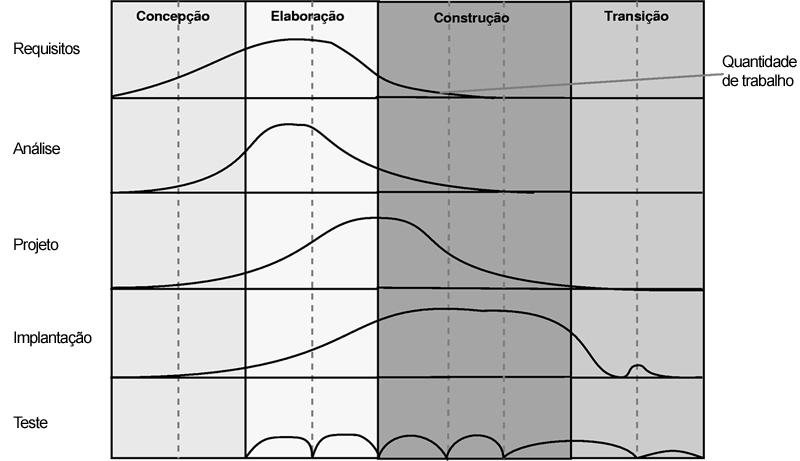
\includegraphics[width=0.8\textwidth]{images/metodologia/fases_workflows.jpg}
            \label{fig:tendencias}
            \caption{Quantidade de trabalho aplicada em cada workflow nas fases do UP \newline {\tiny Fonte: \cite{arlow:2003}}}
        \end{center}
    \end{figure}
\end{frame}

%\begin{frame}
%\frametitle{Metodologia}
%    O UP � iterativo, incremental e dividido em quatro fases:
%
%    \begin{enumerate}
%        \item <2-> Concep��o;
%        \item <3-> Elabora��o;
%        \item <4-> Constru��o;
%        \item <5-> Transi��o.
%    \end{enumerate}
%
%    Cada uma dessas fases � dividida em sub-processos chamados fluxos de trabalho ou \emph{workflows}, s�o eles:
%
%    \begin{itemize}
%        \item <6-> Requisitos;
%        \item <7-> An�lise;
%        \item <8-> Projeto;
%        \item <9-> Implementa��o;
%        \item <10-> Testes.
%    \end{itemize}
%\end{frame}
